\documentclass[a4 paper]{article}
% Set target color model to RGB
\usepackage[inner=2.0cm,outer=2.0cm,top=2.5cm,bottom=2.5cm]{geometry}
\usepackage{setspace}
\usepackage[rgb]{xcolor}
\usepackage{verbatim}
\usepackage{subcaption}
\usepackage{amsgen,amsmath,amstext,amsbsy,amsopn,tikz,amssymb,tkz-linknodes}
\usepackage{fancyhdr}
\usepackage[colorlinks=true, urlcolor=blue,  linkcolor=blue, citecolor=blue]{hyperref}
\usepackage[colorinlistoftodos]{todonotes}
\usepackage{rotating}
\usepackage{hyperref}   % link web
%\usetikzlibrary{through,backgrounds}
\hypersetup{%
pdfauthor={Matteo Azzarelli},%
pdftitle={Homework},%
pdfkeywords={latex, Auditing},%
pdfcreator={PDFLaTeX},%
pdfproducer={PDFLaTeX},%
}
%\usetikzlibrary{shadows}
\usepackage{booktabs}
\newcommand{\ra}[1]{\renewcommand{\arraystretch}{#1}}

\newtheorem{thm}{Theorem}[section]
\newtheorem{prop}[thm]{Proposition}
\newtheorem{lem}[thm]{Lemma}
\newtheorem{cor}[thm]{Corollary}
\newtheorem{defn}[thm]{Definition}
\newtheorem{rem}[thm]{Remark}
\numberwithin{equation}{section}

\newcommand{\homework}[6]{
   \pagestyle{myheadings}
   \thispagestyle{plain}
   \newpage
   \setcounter{page}{1}
   \noindent
   \begin{center}
   \framebox{
      \vbox{\vspace{2mm}
    \hbox to 6.28in { {\bf COMP7015 Artificial Intelligence and Machine Learning \hfill {\small (#2)}} }
       \vspace{6mm}
       \hbox to 6.28in { {\Large \hfill #1  \hfill} }
       \vspace{6mm}
       \hbox to 6.28in { {\it Instructor: {\rm #3} \hfill Name: {\rm #5}, ID: {\rm #6}} }
       %\hbox to 6.28in { {\it TA: #4  \hfill #6}}
      \vspace{2mm}}
   }
   \end{center}
   \markboth{#5 -- #1}{#5 -- #1}
   \vspace*{4mm}
}

\newcommand{\problem}[2]{~\\\fbox{\textbf{Problem #1}}\hfill #2\newline\newline}
\newcommand{\subproblem}[1]{~\newline\textbf{(#1)}}
\newcommand{\D}{\mathcal{D}}
\newcommand{\Hy}{\mathcal{H}}
\newcommand{\VS}{\textrm{VS}}
\newcommand{\solution}{~\newline\textbf{\textit{(Solution)}} }

\newcommand{\bbF}{\mathbb{F}}
\newcommand{\bbX}{\mathbb{X}}
\newcommand{\bI}{\mathbf{I}}
\newcommand{\bX}{\mathbf{X}}
\newcommand{\bY}{\mathbf{Y}}
\newcommand{\bepsilon}{\boldsymbol{\epsilon}}
\newcommand{\balpha}{\boldsymbol{\alpha}}
\newcommand{\bbeta}{\boldsymbol{\beta}}
\newcommand{\0}{\mathbf{0}}

\usepackage{amsmath}

\usepackage{tikz} % draw graph and three
\usetikzlibrary{trees}
\tikzset{
  treenode/.style = {shape=rectangle, rounded corners,
                     draw, align=center},
  root/.style     = {treenode, font=\Large},
  env/.style      = {font=\ttfamily\normalsize},
  dummy/.style    = {treenode}
}




\begin{document}
\homework{Assignment 2}{Due: 8 Apr 2019}{Prof CHEUNG Yiu Ming}{}{Matteo Azzarelli}{18432468}

\problem{Question 1}{}
    \subproblem{a}\\
        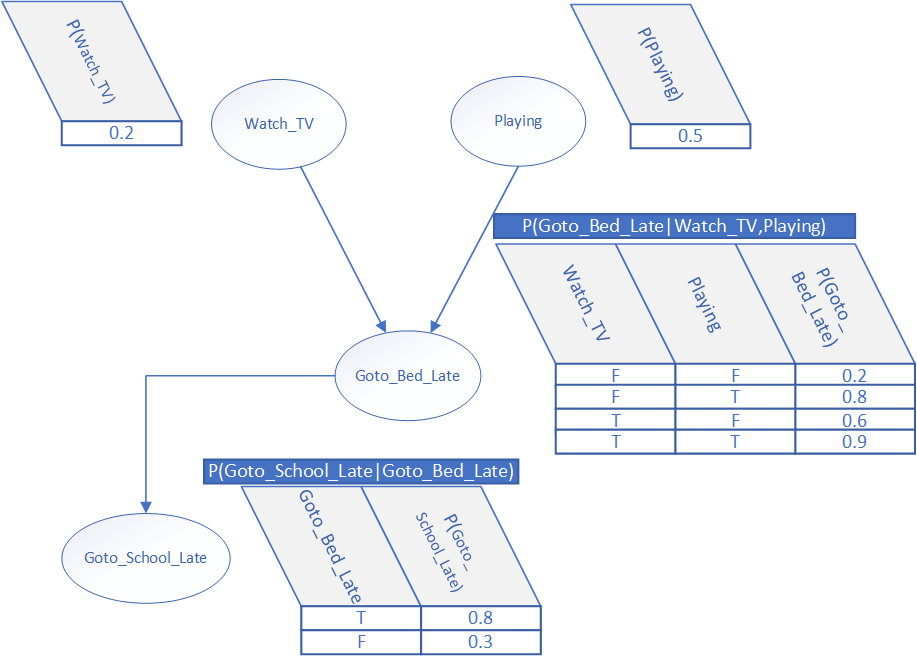
\includegraphics[width=\textwidth]{Exercise1.png}
    \subproblem{b}\\
        \small
        \begin{align*}
            &P(\overline{W} \mid  S , \overline{P}) = \frac{P(\overline{W},S,\overline{P})}{P(S,\overline{P})}=\\
            &=\frac{P(\overline{W},S,\overline{P},B)+P(\overline{W},S,\overline{P},\overline{B}))}
            {P(S,\overline{P},W,B)+P(S,\overline{P},\overline{W},B)+P(S,\overline{P},W,\overline{B})+P(S,\overline{P},\overline{W},\overline{B})}=\\
            &=\frac{P(\overline{W})P(\overline{P})[P(S \mid B)P(B \mid \overline{W},\overline{P})+P(S \mid \overline{B})P(\overline{B} \mid \overline{W},\overline{P})]}
            {P(W)P(\overline{P})[P(S \mid B)P(B \mid W,\overline{P}) + P(S \mid \overline{B})P(\overline{B} \mid W,\overline{P}) ] + P(\overline{W})P(\overline{P})[P(S \mid B)P(B \mid \overline{W},\overline{P}) + P(S \mid \overline{B})P(\overline{B} \mid \overline{W},\overline{P}) ]}=\\
            &=\frac{0.8 \cdot 0.5 \cdot [0.8 \cdot 0.2 + 0.3 \cdot 0.8]}{0.2 \cdot 0.5 \cdot [0.8 \cdot 0.6 + 0.3 \cdot 0.4] + 0.8 \cdot 0.5 \cdot [0.8 \cdot 0.2 + 0.3 \cdot 0.8]}= \frac{0.16}{0.22}= 0.\overline{72}
        \end{align*}
        \normalsize    
\newpage
\problem{Question 2}{}
    
    1) Calculate the Entropy of the target (\textbf{Risk}):\\
        Risk has three possible value: high~(h = 6), moderate~(m = 3), low~(l = 5)
        \begin{flalign*}
            E(S) &= -\frac{h}{h+m+l}\log_{2}{\left (\frac{h}{h+m+l} \right )} -\frac{m}{h+m+l}\log_{2}{\left ( \frac{m}{h+m+l} \right )}-\frac{l}{h+m+l}\log_{2}{\left (\frac{l}{h+m+l} \right )}=\\
            &=-\frac{6}{14}\log_{2}{\left (\frac{6}{14}  \right )}-\frac{3}{14}\log_{2}{\left (\frac{3}{14}  \right )}-\frac{5}{14}\log_{2}{\left (\frac{5}{14}  \right )}= 1.531
        \end{flalign*}
        
    2) Calculate the information gain of each attribute. So in order to do that we have to calculate the entropy of each subset of that attribute.
        
        $$IG(S, A_{i}) = E(S) - \sum_{t \in T_i}{\left(\frac{\mid t \mid}{\mid S \mid}E(t)\right)}$$
    where $T_i$ is the set of subset created from splitting $S$ by attribute $A_i$.
    
    % Credit History
    Calculate the Information Gained for \textbf{Credit History}, first of all calculate the entropy for \textit{good}, \textit{bad} and \textit{unknown}. Among the 14 customers, 5 are \textit{good} and 1 of them is \textit{High risk}, 1 is \textit{Moderate risk} and 3 are \textit{Low risk}, so:
    
    \begin{equation*}
        E(good) = -\frac{1}{5}\log_{2}{\left (\frac{1}{5} \right )} -\frac{1}{5}\log_{2}{\left ( \frac{1}{5} \right )}-\frac{3}{5}\log_{2}{\left (\frac{3}{5} \right )}= 1.371
    \end{equation*}
    \textit{bad} has 4 value, 3 are \textit{high risk} and 1 is \textit{moderate risk}.
    \begin{equation*}
        E(bad) = -\frac{3}{4}\log_{2}{\left (\frac{3}{4} \right )} -\frac{1}{4}\log_{2}{\left ( \frac{1}{4} \right )}= 0.811
    \end{equation*}
    \textit{unknown} has 5 value, 2 are \textit{high risk}, 1 is \textit{moderate risk} and 2 are \textit{low risk}.
    \begin{equation*}
        E(unknown) = -\frac{2}{5}\log_{2}{\left (\frac{2}{5} \right )} -\frac{1}{5}\log_{2}{\left ( \frac{1}{5} \right )}-\frac{2}{5}\log_{2}{\left (\frac{2}{5} \right )}= 1.522
    \end{equation*}
    
    Calculate the Information Gain of Credit History
    \begin{flalign*}
        IG(S, Credit History) &= E(S) - \frac{5}{14}E(good) - \frac{4}{14}E(bad) - \frac{5}{14}E(unknown) =\\
        &= 1.531 - \frac{5}{14}1.371 - \frac{4}{14}0.811 - \frac{5}{14}1.522 = \textbf{0.266}
    \end{flalign*}
    
    % Debt
    Information gain \textbf{Debt}:\\
    \textit{high} has 7 value, 4 are \textit{high risk}, 1 is \textit{moderate risk} and 2 are \textit{low risk}.
    \begin{equation*}
        E(high) = -\frac{4}{7}\log_{2}{\left (\frac{4}{7} \right )} -\frac{1}{7}\log_{2}{\left ( \frac{1}{7} \right )}-\frac{2}{7}\log_{2}{\left (\frac{2}{7} \right )}= 1.379
    \end{equation*}
    \textit{low} has 7 value, 2 are \textit{high risk}, 2 are \textit{moderate risk} and 3 are \textit{low risk}.
    \begin{equation*}
       E(low) = -\frac{2}{7}\log_{2}{\left (\frac{2}{7} \right )} -\frac{2}{7}\log_{2}{\left ( \frac{2}{7} \right )}-\frac{3}{7}\log_{2}{\left (\frac{3}{7} \right )}= 1.557
    \end{equation*}
    
    \begin{flalign*}
        IG(S, Debt) &= E(S) - \frac{7}{14}E(high) - \frac{7}{14}E(low) =\\
        &= 1.531 - \frac{7}{14}1.379 - \frac{7}{14}1.557 = \textbf{0.063}
    \end{flalign*}
    
    \newpage
    % Income
    Information gain \textbf{Income}:\\
    \textit{\$0 to \$15k} has 4 value, all of them are \textit{high risk}.
    \begin{equation*}
        E(\$0 to \$15k) = -\frac{4}{4}\log_{2}{\left (\frac{4}{4} \right )} = 0
    \end{equation*}
    \textit{\$15k to \$35k} has 4 value, 2 are \textit{high risk} and 2 are \textit{moderate risk}.
    \begin{equation*}
       E(\$15k to \$35k) = -\frac{2}{4}\log_{2}{\left (\frac{2}{4} \right )} -\frac{2}{4}\log_{2}{\left ( \frac{2}{4} \right )} = 1
    \end{equation*}
    \textit{over \$35k} has 6 value, 1 are \textit{moderate risk} and 5 are \textit{low risk}.
    \begin{equation*}
       E(over \$35k) = -\frac{1}{6}\log_{2}{\left ( \frac{1}{6} \right )}-\frac{5}{6}\log_{2}{\left (\frac{5}{6} \right )}= 0.65
    \end{equation*}
    
    \begin{flalign*}
        IG(S, Debt) &= E(S) - \frac{4}{14}E(\$0 to \$15k) - \frac{4}{14}E(\$15k to \$35k) - \frac{7}{14}E(over \$35k) =\\
        &= 1.531 - \frac{4}{14}0 - \frac{4}{14}1 - \frac{6}{14}0.65 = \textbf{0.967}
    \end{flalign*}
    
    The attribute \textit{income} is the greatest one with $0.967$, so it became the root node of decision tree with three branches as \textit{over \$35k}, \textit{\$15k to \$35k} and \textit{\$0 to \$15k}.
    
    Now we are going to build the next level of the decision tree.
    //
    We start with the \textit{over \$35k} branch:
    
    Information gain \textbf{Credit history}:
    because all customer that has high income(\textit{over \$35k}) and good credit is classified as low risk, $E(good) = 0$, and is the same for $E(bad)$ and $E(unknown)$ because all of them are classified in the same cluster.
    So the information gain form \textbf{Credit History} is:
    
    \begin{flalign*}
        IG(S_{over \$35k}, Credit History) &= E({over \$35k}) - \frac{3}{6}0 - \frac{1}{6}0 - \frac{2}{6}0 = 0.65
    \end{flalign*}
    
    Information gain \textbf{Debt}:
    
    \begin{equation*}
       E(low) = -\frac{3}{4}\log_{2}{\left ( \frac{3}{4} \right )}-\frac{1}{4}\log_{2}{\left (\frac{1}{4} \right )}= 0.811
    \end{equation*}
    And $E(high) = 0$ because all of them is in the same class.
    
    So the Informaiton gain is:
    \begin{flalign*}
        IG(S_{over \$35k}, Debt) &= E({over \$35k}) - \frac{4}{6}E(low) - \frac{2}{6}0 = 0.65 - \frac{4}{6}0.811 = 0.109
    \end{flalign*}
    
    Because the information gain from \textit{Credit history} is the greatest on this will became the next level of the decision tree and since the entropy for each branch is zero, the tree is not growing anymore in this direction.\\
    $\textbf{good}~and~\textbf{unknown} \longrightarrow low risk$\\
    $\textbf{bad} \longrightarrow high risk$\\
    
    
    
    Now\textit{\$15k to \$35k} branch:
        Information gain \textbf{Credit history}:\\
        $E(good) = 0$ and $E(bad) = 0$,
        
        \begin{equation*}
            E(unknown) = -\frac{1}{2}\log_{2}{\left ( \frac{1}{2} \right )}-\frac{1}{2}\log_{2}{\left (\frac{1}{2} \right )}= 1
    \end{equation*}
    
    So, the information gain is:
    
    \begin{flalign*}
        IG(S_{\$15k to \$35k}, Debt) &= E({\$15k to \$35k}) - \frac{1}{4}0 - \frac{2}{4}E(unknown) - \frac{1}{4}0=\\
        &= 1 - \frac{2}{4}1 = 0.5
    \end{flalign*}
    \\
    Information gain \textbf{Debt}:
        $E(low) = 0$,
        
        \begin{equation*}
            E(high) = -\frac{2}{3}\log_{2}{\left ( \frac{2}{3} \right )}-\frac{1}{3}\log_{2}{\left (\frac{1}{3} \right )}= 0.918
        \end{equation*}
        
         So, the information gain is:
         
         \begin{flalign*}
        IG(S_{\$15k to \$35k}, Debt) &= E({\$15k to \$35k}) - \frac{1}{4}0 - \frac{3}{4}E(high)=\\
        &= 1 - \frac{3}{4}0.918 = 0.3115
    \end{flalign*}
    
    The information gain from Credit history is the grater one so it will became the next level of this branch.\\
    
    For the \textit{\$0 to \$15k} branch we cant split any more, so it assume the value high risk.\\
    
    Now we continue with the only remained branch, \textit{\$15k to \$35k} and \textit{unknown}.
    If is $\textbf{high} \longrightarrow \textit{high risk}$, if is $\textbf{low} \longrightarrow \textit{moderate risk}$.
    
    The final decision tree is showed in fig.~\ref{fig:DecisionTree}:\\
    \begin{figure}[h]
        \centering
        \begin{tikzpicture}
            [   grow= circle,
                level distance=5cm,
                level 1/.style={sibling distance=5cm},
                level 2/.style={sibling distance=2cm}]
            \node [root] {Income}
                child { node [dummy] {Credit History}
                    child{node {Low Risk}
                        edge from parent node [below] {good}
                    }
                    child{node {Low Risk}
                        edge from parent node [below] {unknown}
                    }
                    child{node {Moderate Risk}
                        edge from parent node [below] {bad}
                    }
                    edge from parent node [below] {over \$35k}
                }
                child { node [dummy] {Credit History}
                    child{node {Moderate Risk}
                        edge from parent node [below] {good}
                    }
                    child{node {High Risk}
                        edge from parent node [below] {bad}
                    }
                    child{node [dummy]{Debt}
                        child{node {Moderate Risk}
                        edge from parent node [below] {low}
                    }
                    child{node {High Risk}
                        edge from parent node [below] {high}
                    }
                        edge from parent node [below] {unknown}
                    }
                    edge from parent node [below] {\$15k to \$35k}
                }
                child { node [] {High Risk}
                    edge from parent node [below] {\$0 to \$15k}
                };
            
        \end{tikzpicture}
        
        \caption{Decision tree}
        \label{fig:DecisionTree}
    \end{figure}
    
\newpage
\problem{Question 3}{}
    \subproblem{a}
        $$P(\textbf{Risk}=low) = \frac{5}{14} = 0.357$$
        $$P(\textbf{Risk}=moderate) = \frac{3}{14} = 0.214$$
        $$P(\textbf{Risk}=high) = \frac{6}{14} = 0.429$$
        
    \subproblem{b}
        Given the new entry:\\
        \textbf{Credit History}(\textbf{CH}) = bad, \textbf{Debt}(\textbf{D}) = low, \textbf{Income}(\textbf{I}) = \$0 to \$15k
        \begin{flalign*}
            &P(\textbf{Risk}=low)
            P(\textbf{CH} = bad \mid \textbf{R}=low)
            P(\textbf{D} = low \mid \textbf{R}=low)
            P(\textbf{I} = \$0 to \$15k \mid \textbf{R}=low) =\\
            = &P(\textbf{R}=low) 
            \left( {\frac{P(\textbf{CH} = bad \wedge \textbf{R}=low)}{P(\textbf{R}=low)}} \right)
            \left( {\frac{P(\textbf{D} = low \wedge \textbf{R}=low)}{P(\textbf{R}=low)}} \right)
            \left( {\frac{P(\textbf{I} = \$0 to \$15k \wedge \textbf{R}=low)}{P(\textbf{R}=low)}} \right) = 0
        \end{flalign*}
        Since $P(\textbf{CH} = bad \wedge \textbf{R}=low) = 0$ and $P(\textbf{I} = \$0 to \$15k \wedge \textbf{R}=low) = 0$, follow that the multiplication is 0. 
        
        \begin{flalign*}
            &P(\textbf{Risk}=moderate)
            P(\textbf{CH} = bad \mid \textbf{R}=moderate)
            P(\textbf{D} = low \ mid \textbf{R}=moderate)
            P(\textbf{I} = \$0 to \$15k \mid \textbf{R}=moderate) =\\
            = &P(\textbf{R}=mod) 
            \left( {\frac{P(\textbf{CH} = bad \wedge \textbf{R}=mod)}{P(\textbf{R}=mod)}} \right)
            \left( {\frac{P(\textbf{D} = low \wedge \textbf{R}=mod)}{P(\textbf{R}=mod)}} \right)
            \left( {\frac{P(\textbf{I} = \$0 to \$15k \wedge \textbf{R}=mod)}{P(\textbf{R}=mod)}} \right) = 0
        \end{flalign*}
        Since $P(\textbf{CH} = bad \wedge \textbf{R}=low) = 0$ and $P(\textbf{I} = \$0 to \$15k \wedge \textbf{R}=low) = 0$, follow that the multiplication is 0.
        
        \begin{flalign*}
            &P(\textbf{Risk}=high)
            P(\textbf{CH} = bad \mid \textbf{R}=high)
            P(\textbf{D} = low \ mid \textbf{R}=high)
            P(\textbf{I} = \$0 to \$15k \mid \textbf{R}=high) =\\
            = &P(\textbf{R}=high) 
            \left( {\frac{P(\textbf{CH} = bad \wedge \textbf{R}=high)}{P(\textbf{R}=high)}} \right)
            \left( {\frac{P(\textbf{D} = low \wedge \textbf{R}=high)}{P(\textbf{R}=high)}} \right)
            \left( {\frac{P(\textbf{I} = \$0 to \$15k \wedge \textbf{R}=high)}{P(\textbf{R}=high)}} \right) =\\
            = &\frac{6}{14}
            \left( {\frac{\frac{3}{14}}{\frac{6}{14}}} \right)
            \left( {\frac{\frac{2}{14}}{\frac{6}{14}}} \right)
            \left( {\frac{\frac{4}{14}}{\frac{6}{14}}} \right)
            = \frac{6}{14}
            \left( {\frac{3}{6}} \right)
            \left( {\frac{2}{6}} \right)
            \left( {\frac{4}{6}} \right) = \textbf{0.048}
        \end{flalign*}
        
        So, the new instance is classified as \textbf{\textit{High Risk}}.
\end{document} 


